\documentclass[10pt,twocolumn,letterpaper]{article}
%% Welcome to Overleaf!
%% If this is your first time using LaTeX, it might be worth going through this brief presentation:
%% https://www.overleaf.com/latex/learn/free-online-introduction-to-latex-part-1

%% Researchers have been using LaTeX for decades to typeset their papers, producing beautiful, crisp documents in the process. By learning LaTeX, you are effectively following in their footsteps, and learning a highly valuable skill!

%% The \usepackage commands below can be thought of as analogous to importing libraries into Python, for instance. We've pre-formatted this for you, so you can skip right ahead to the title below.

%% Language and font encodings
\usepackage[brazil]{babel}
\usepackage[utf8x]{inputenc}
\usepackage[T1]{fontenc}
\usepackage{verbatim}

%% Sets page size and margins
\usepackage[a4paper,top=3cm,bottom=2cm,left=3cm,right=2cm,marginparwidth=1.75cm]{geometry}

%% Useful packages
\usepackage{amsmath}
\usepackage{graphicx}
\usepackage[colorinlistoftodos]{todonotes}
\usepackage[colorlinks=true, allcolors=blue]{hyperref}
\usepackage[numbers]{natbib}
\bibliographystyle{IEEEtranN}
%% Title
\title{
		\usefont{OT1}{bch}{b}{n}
		\normalfont \normalsize \textsc{EEL7323-08235 Programação C++ para Sistemas Embarcados} \\ [10pt]
		\huge Bússola eletrônica de 2 eixos \\
}
\selectlanguage{english}
\usepackage{authblk}
\renewcommand\Authand{, e }
\renewcommand\Authands{, e }
\author[1]{Gustavo Batistell}
\affil[1]{UFSC - Universidade Federal de Santa Catarina \\
\newline Curso de Graduação em Engenharia Eletrônica}

\begin{document}
\maketitle

\section{Introdução}

O objetivo deste projeto é desenvolver um magnetômetro eletrônico capaz de apresentar, entregar e salvar os dados de \emph{heading}, 
ou direção em relação ao campo magnético terrestre, ou seja, a direção apontada pelo equipamento.
Os magnetômetros eletrônicos são parte importante na instrumentação de embarcações, aeronaves, submarinos, satélites, etc e durante 
a realização do estágio no Laboratório do Grupo Drakkar Atlantec em Florianópolis, foi constatada a demanda para dominar tanto o 
ajuste quanto a calibração deste tipo de instrumento. Apesar da empresa contar com as boninas de Helmhotz com controlador e um 
magnetômetro  de referência, tanto a parte eletrônica quanto os softwares embarcados carecem de atualização, melhoria e nova 
implementação para completo domínio do funcionamento. Essa necessidade de dominar (novamente) por completo o sistema surgiu devido 
perda de documentação e dos códigos originais com o passar dos anos. \\
Para isso, a tarefa do desenvolvimento inicial foi dividida em duas partes: uma parte para acionamento (driver) e outra parte para 
um magnetômetro, este último no qual fiquei incumbido.\\
Assim, utilizado um módulo micro-controlado ARM RP2040 Raspberry Pi Pico \cite{RP2040_Datasheet}, um módulo magnetômetro para medir 
o campo magnético em pelo menos 2 eixos (seja o HMC5883 ou HoneyWell HMR3300 \cite{HMR3300_Datasheet} disponíveis no laboratório), realizar o acionamento 
de leds para apresentar o \emph{heading}, realizar log de dados e suportar acesso via UART/USB e Wireless. Ver diagrama da 
\autoref{fig:Diagrama_blocos}.

\begin{figure}[ht]
  \centering
  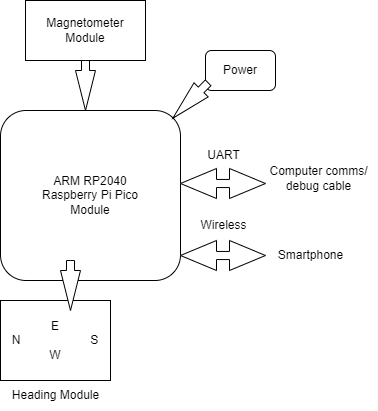
\includegraphics[width=\linewidth]{figures/ProjetoFinalCPP_Diagrama.png}
  \caption{Diagrama de blocos revisado do projeto.}
  \label{fig:Diagrama_blocos}
\end{figure}

\section{Requisitos}

Os requisitos de projeto foram combinados com a demanda do Laboratório do Grupo Drakkar Atlantec e as 
especificações solicitadas pelo professor, aproveitando-se da portabilidade e modularidade com a 
linguagem de programação C++ e os conceitos de orientação a objetos, polimorfismo, classes, etc. Assim, 
foram listados os requisitos de desenvolvimento combinados para uma Bússola Eletrônica conforme segue:

\begin{itemize}
    \item Apresente em mostrador simples de LEDs o \emph{heading} em 8 direções: N, NE, E, SE, S, SW, W e NW.
    \item Utilize um módulo de magnetômetro de pelo menos 2 eixos (seja analógico ou digital) para obtenção 
    das componentes de campo magnético.
    \item Com as componentes X e Y de campo magnético calcular a direção (em graus de 0 a 360) que também 
    pode ser utilizada para o \emph{heading}.
    \item Realizar log da ID, timeStamp e dados.
    \item Aceitar a consulta e envio deste log para um \emph{host}.
    \item Aceitar comunicação via UART/USB.
    \item Aceitar comunicação \emph{wireless}.
    \item O \emph{host} pode conferir a listagem do log.
    \item O \emph{host} pode conferir o tempo em que a Bússola Eletrônica se manteve ativa 
\end{itemize}

\section{Design Proposto do sistema embarcado}

Como o microcontrolador ARM RP2040 \cite{RP2040_Datasheet} é \emph{dual-core} foi decidido implementar 2 máquinas de estado. Uma 
delas para a aplicação da Bússola Eletrônica propriamente dita, que ao ser iniciada segue diretamente para o estado de aquisição 
de dados brutos, depois para um estado que calcula a direção a partir das componentes X e Y dos dados brutos, outro estado que 
armazena o log e finalmente um estado que exibe o \emph{heading}. Essa primeira máquina de estados na \emph{Trhead 1} é apresentada
na \autoref{fig:maquina_estados1} e é importante destacar a importância dela na gravação/escrita em RAM.
\begin{figure}[h]
  \centering
  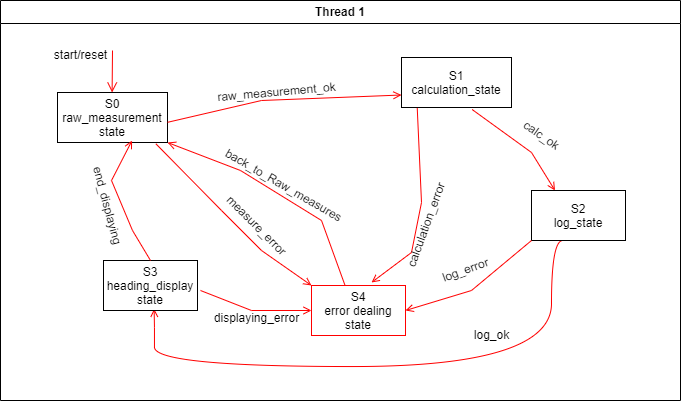
\includegraphics[width=\linewidth]{figures/maquina_estados1.png}
  \caption{Maquina de estados principal (com gravação em memória).}
  \label{fig:maquina_estados1}
\end{figure}
Já a segunda máquina de estados na \emph{Trhead 2} é incumbida de controlar a conectividade UART e \emph{Wireless}, conforme mostrado 
na a \autoref{fig:maquina_estados2}. Esta máquina de estados tem um estado de \emph{idle} para quando não houver conexão, um estado 
para conexão \emph{wireless} estabelecida, um estado para o wirelessRequest, um estado para quando a conexão UART é estabelecida, um 
estado para o UARTrequest e um estado para tratamento de erros. Esta máquina desta \emph{Trhead 2} apenas acessa os dados. Essa 
distinção entre gravação e acesso deste projeto em específico é importante para evitar problemas de leitura e escrita usuais em 
programação concorrente quando mais de uma \emph{trhead} é possível.
\begin{figure}[h]
  \centering
  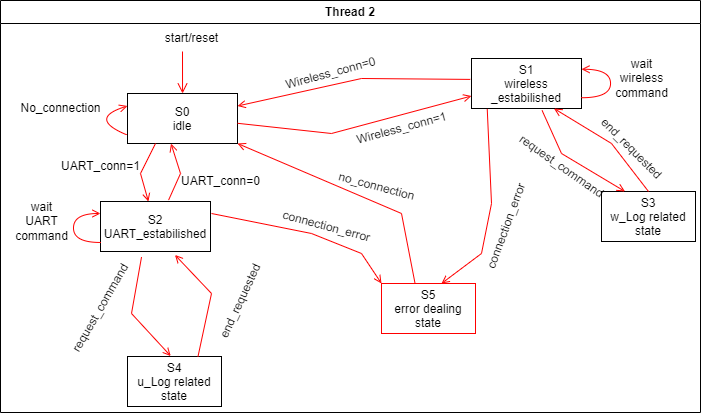
\includegraphics[width=\linewidth]{figures/maquina_estados2.2.png}
  \caption{Maquina de estados secundária para conexões UART e Wireless (apenas acesso a memória).}
  \label{fig:maquina_estados2}
\end{figure}

%\begin{figure}
%  \centering
%  \includegraphics[width=\linewidth]{figures/Tabela-de-estados.png}
%  \caption{Tabela de estados.}
%\end{figure}

Para garantir a modularidade do projeto, o diagrama de classes proposto utilizou de 5 níveis gerais (com uma subdivisão para a camada de drivers externos e \emph{on-board} incluída em revisão) de abstração que são listados abaixo em uma abordagem "de dentro para fora":
\begin{itemize}
  \item Hardware Abstraction Layer (HAL): Responsável por abstrair o hardware subjacente, incluindo os módulos do SDK da Raspberry Pi Pico.
  \item Device Drivers Layer: Essa camada mais geral foi subdivididida após revisão, pois gerencia os drivers para GPIO, UART, comunicação sem fio (que são \emph{on-board} da Raspberry Pi Pico) e o magnetômetro (que é um dispositivo externo à Raspberry Pi Pico, por isso locado na subcamada de drivers externos).
  \item Processing Layer: Lida com o processamento dos dados, incluindo a classe `DirectionCalculator`. Esta camada também pode ser usada 
  para implementações futuras de técnicas de Digital Signal Processing como média móvel, dizimação, etc.
  \item Control/Application Layer: Responsável por controlar as partes funcionais do projeto. É o ponto central onde as operações 
  funcionais são coordenadas, incluindo as classes `HeadingDisplay', `Log', `UART' e `Wireless'. 
  \item User Interaction Layer: É a camada mais externa que lida com a interação do usuário, onde está a classe ``ElectronicCompass'' propriamente dita.
\end{itemize}
Essa organização se apresentou clara e permite uma separação adequada de responsabilidades em cada camada de classes do sistema, 
o que é uma boa prática para melhor documentar, estruturar e facilitar a compreensão e manutenção do projeto. O diagrama de classes 
pode ser visto na \autoref{fig:diagrama-classes} do no Apêndice A.

\section{Design Proposto para o \emph{Host}}
A proposta para o \emph{Host} é implementar um software que deve rodar no computador, na máquina 
virtual WSL Ubuntu, apresentar um menu na tela em que um usuário ADMIN possa: escolher algumas das opções 
apresentadas pressionando a tecla específica no teclado+<enter>; o software envia pela USB (porta COM) e recebe
comandos e dados, respectivamente, do sistema embarcado externo a esse computador que usa a UART a 115200 kbps.\\
Quando o software é iniciado, o usuário ADMIN deve confirmar o início da conexão, e pode escolher da lista do menu: 
\begin{itemize}
  \item listar e pegar todos os eventos ocorridos em um determinado intervalo de datas; 
  \item obter o tempo total em hh:mm que o controlador esteve ativo;
  \item listar e pegar os eventos instantâneos (\emph{real time});
  \item desativar conexão/sair.
\end{itemize}

Usando o mesmo conceito de camadas para o projeto do software do \emph{Host}, o diagrama de classes é apresentado na \autoref{fig:diagrama-host} do Apêndice B. 
Dessa maneira, a modularidade do projeto no \emph{Host} também é facilitada, por exemplo se houver interesse em implementar o sistema para outro módulo como STM32 ao invés da Raspberry Pi Pico. 
A descrição das camadas é parecida com o que já foi descrito para o projeto embarcado, de dentro para fora:
\begin{itemize}
  \item Device Drivers Layer: Essa camada mais geral gerencia os drivers para comunicação com a Raspberry e o driver da serial port.
  \item Control/Application Layer: Responsável por controlar o equipamento e os dados/comandos de saída/entrada. É o ponto central onde as operações 
  funcionais são coordenadas. 
  \item User Interaction Layer: É a camada mais externa que lida com a interação do usuário, e sua interface com o software.
\end{itemize}

\section{Resultados de implementação}
A execução do projeto como um todo levou em consideração o uso das técnicas apresentadas em aula. 
Os exemplos apresentados a seguir constam em trechos dos códigos disponíveis no repositório do GitHub\cite{src-github}. 

\subsection{Uso de Herança e Herança Múltipla}
No decorrer do projeto o uso de Herança foi exencial, por exemplo nas classes Connection e PicoConnection do projeto do \emph{Host}, mas certamente o exemplo mais notável é de Herança Múltipla nas classes base Clock e Calendar e na classe derivada ClockCalendar. A classe ClockCalendar herda publicamente tanto de Clock quanto de Calendar, indicando a Herança Múltipla, como pode ser visto no trecho de código abaixo: 
{\scriptsize
\begin{verbatim}
  #include "ClockCalendar.hpp"

  ClockCalendar::ClockCalendar(int t_day, int t_month, 
                int t_year, int t_hr, int t_min, int t_sec, 
                int t_isPm)
      : Clock(t_hr, t_min, t_sec, t_isPm), Calendar(t_day, 
              t_month, t_year) {
      // Inicializa classe base Clock c.parametros de tempo
      // Inicializa classe base Calendar c.parametros de data
  }
  
  void ClockCalendar::advance() {
      // Implementacao de advance() para classe ClockCalendar
      // chamar advance() das classes base Clock e Calendar
  }
\end{verbatim}
}

\subsection{Uso de Friends}
Um exemplo de uso de Friends, que é uma forma de permitir que uma classe ou uma função acesse os membros privados ou protegidos de outra classe, sem violar o princípio do encapsulamento, foi utilizado nas classes Connection e Data do projeto do \emph{Host}. 
Essa implementação pode ser vista nos códigos fonte dos arquivos Connection.h, Data.h e Data.cpp. Abaixo segue recorte do arquivo Connection.h mostrando o uso de Friends (notar que trechos do código considerados irrelevantes para o exemplo foram omitido com ``...''):
{\scriptsize
\begin{verbatim}
  /**
  * *****************************************************,
  * File:       Connection.h
  ...
  public:
  ...
    friend class Data;
    //Declara classe Data como amiga para
    //acessar membros privados de Connection
    
    queue<string> dataQueue; 
    // Fila para armazenar dados recebidos pela serial
    // declarada como pública para classe Data acessar

...  
\end{verbatim}
}

\subsection{Uso de Template}
Um template pode ser útil para evitar a repetição de código ou para implementar algoritmos independentes de tipos. 
Um exemplo de uso de template pode ser visto no projeto do \emph{Host}, especificamente na classe Data, que usa um template para definir o método chamado saveData, que salva os dados da fila dataQueue em um arquivo de texto, com qualquer tipo de dado que possa ser convertido em string.
Segue trecho do código citado: 
{\scriptsize
\begin{verbatim}
  ...
template <typename T>
void Data::saveData(queue<T> dataQueue) {
    ofstream file; 
    // Cria objeto classe ofstream para saida
    
    file.open("data.txt"); 
    // Abre o arquivo data.txt
    
    if (file.is_open()) { 
      // Se aberto com sucesso

        while (!dataQueue.empty()) { 
          // Enquanto fila dataQueue não vazia

            file << dataQueue.front() << endl; 
            // Escreve elemento da frente da 
            //fila no arquivo com quebra de linha

            dataQueue.pop(); 
            // Remove o elemento da frente da fila
        }
        file.close(); 
        // Fecha o arquivo

        cout << "Dados salvos com sucesso." << endl;
    }
    else { 
      // Se arquivo não aberto
        cout << "Erro ao abrir o arquivo." << endl;
    }
    ...
}

\end{verbatim}
}

\subsection{Uso de Funções Virtuais}
As funções virtuais são funções ou métodos cujo comportamento pode ser sobrescrito em uma classe herdeira por uma função com a mesma assinatura e são parte fundamental para funcioanmento do conceito de Polimorfismo Abstrato.
Um exemplo de uso de Funções virtuais no projeto do \emph{Host} pode ser visto nos códigos dos arquivos Connection.h e PicoConnection.h abaixo, respectivamente. Abaixo seguem recortes dos arquivos mostrando o uso (notar que trechos do código considerados irrelevantes para o exemplo foram omitido com ``...''):
{\scriptsize
\begin{verbatim}
    ...
    #include <string>
    #include "PicoConnection.h" 
    // Arquivo cabeçalho da classe PicoConnection
    
    #include "SerialPort.h" 
    // Arquivo de cabecalho da classe SerialPort
    #include...
      ...
      class Connection {
      private:
      ...
      public:
      ...
          virtual void send(string message); 
          // para enviar mensagem pela serial
          
          virtual string receive(); 
          // para receber mensagem pela porta serial
    }
  \end{verbatim}
}  
{\scriptsize
\begin{verbatim}
    ...
  
  #include <string>
  #include "Connection.h" 
  // arquivo de cabeçalho da classe Connection
     ...
   
     class PicoConnection 
     ...
       private:
       ...
       public:
       ...
       void send(string message) override; 
       // para enviar comando pela serial

       string receive() override; 
       // para receber resposta pela serial
       ...
  ...  
\end{verbatim}
}

\subsection{Uso do Tratamento de Exceções}
Tratamento de exceções é um recurso que permite lidar com situações de erro ou anormais e sua aplicação consiste no uso de três palavras-chave: try, throw e catch.
No trecho de código abaixo da classe DirectionCalculator do projeto embarcado é apresentada uma solução pra tratamento da exceção de divisão por zero:

{\scriptsize
\begin{verbatim}
  // Metodo para calcular direcao com dados brutos
  void DirectionCalc::calculateDirection() {

      // Simulacao de calculos 
      rawX = 1.0;  
      rawY = 2.0;
  
      // bloco try-catch para tratar a excecao
      try {

          // Verifica se os dados brutos sao validos
          if (rawX <= 0 || rawY <= 0) {

              // Lanca uma excecao com a mensagem
              throw "Dados brutos inválidos";
          }
          else {

              // Realiza calculos para obter a direcao
              // (trecho em implementação)
              double calculatedDirection = rawX + rawY;
  
              // Atualiza o log com dados 
              updateLog("Direction calculated: " 
                + std::to_string(calculatedDirection));
          }
      }
      catch (const char* msg) {
        
          // Captura a excecao se for uma string
          // Mostra a mensagem de erro
          cerr << "Erro: " << msg << endl;
      }
  }
 int main() {

    // Cria objeto da classe Log
    Log log;

    // Cria objeto DirectionCalc e passa log como parametro
    DirectionCalc dc(log);

    // bloco try-catch para tratar a excecao
    try {

        // Chama o metodo calculateDirection do objeto dc
        dc.calculateDirection();
    }
    catch (const char* msg) {

        // Captura a excecao se for uma string
        // Mostra a mensagem de erro
        cerr << "Erro: " << msg << endl;
    }
    catch (...) {

        // Captura qualquer outra excecao
        // Mostra mensagem erro
        cerr << "Erro desconhecido" << endl;
    }
    return 0;
}
...
\end{verbatim}
}

\subsection{Uso de sobrecarga de operadores}
Um exemplo de sobrecarga do operador de inserção ``<<'' (que pode ajudar a organizar a estrutura e comprimento do código) foi utilizado para a inserção de registro à fila da classe Log do projeto embarcado:
{\scriptsize
\begin{verbatim}
  #ifndef LOG_H
  #define LOG_H
  
  #include <queue>
  #include <string>
  #include "Compass.h"        // Inclui classe Compass
  #include "DirectionCalc.h"  // Inclui classe DirectionCalc
  #include "UART.h"           // Inclui classe UART/USB
  #include "Wireless.h"       // Inclui classe Wireless
  
  class Log {
  public:
      // Construtor aceita objetos relacionados 
      //como parametros
      Log(Compass& compass, DirectionCalc& directionCalc, 
          UART& uart, Wireless& wireless);
  
      // Sobrecarga do operador << para adicionar log fila
      Log& operator<<(const std::string& logData);
      }  
\end{verbatim}
}

\subsection{Uso de Polimorfismo com Classes Abstratas}
O Polimorfismo é um princípio fundamental na Programação Orientada a Objetos e envolve o uso conjunto de Herança e Funções Virtuais, 
permitindo que classes derivadas de uma única classe base invoquem métodos com a mesma ``assinatura'', mas que se comportam de maneira diferente para cada uma das classes derivadas. 
De fato, neste projeto o uso de funções virtuais e herança, caracterizam o emprego de polimorfismo com classes abstratas. Por exemplo na classe base Connection e classe derivada PicoConnection do projeto do \emph{Host} já exemplificadas acima na subseção ``Uso de Funções Virtuais''.


\subsection[short]{Implementação de lista e fila (\emph{Queue})}
Os eventos da fila com ID do sistema embarcado, data/hora do evento usando o 
ClockCalendar foram implementados na clase Log do projeto embarcado e a lista do projeto do \emph{Host} já teve implementação apresentada acima no subitem Uso de Template, onde também foi implementada a limpeza da fila quando log é transferido para o \emph{host}.
%\subsection[short]{Implementação da comunicação UART/USB}

\subsection[short]{Implementação da Wireless}
Apesar de dessa parte do projeto não ser mais requisito, ela tem menção em vários trechos do projeto e facilmente pode ser retomada utilizando o próprio WirelessDriver disponível em algumas versões da Raspberry Pi Pico, entrando na parte do projeto embarcado na camada Onboard Drivers Layer.
A outra ``ponta'' da comunicação wireless pode ser um smartphone Android com software projetado nos mesmos moldes do projeto de software do \emph{Host}.
\subsection[short]{Montagem dos módulos/circuitos}
A montagem dos módulos foi realizada em protoboard conforme a \autoref{fig:montagem} do Apêndice C. Mais a esquerda na imagem encontra-se o módulo magnetômetro HoneyWell \cite{HMR3300_Datasheet}. 
Foi implementado circuito com transistores para ajustar as tensões de 3.3V e 5V entre as conexões SPI do módulo magnetômetro \cite{HMR3300_Datasheet} e a Raspberry Pi Pico \cite{RP2040_Datasheet}.
Mais ao centro da imagem está o módulo Raspberry Pi Pico \cite{RP2040_Datasheet} rodeado pelos 8 LEDs previstos para indicação da direção (\emph{heading}).
Mais a direita da imagem o módulo em vermelho está um conversor UART-USB da FTDI. 

\section{Conclusões}
A organização do projeto de sistemas embarcados por blocos funcionais e, principalmente, por diagrama de 
classes disposto em camadas, é certamente uma das principais vantagens constatadas no decorrer deste trabalho. 
A abstração necessária para isso pode tomar certo tempo para ser desenvolvida, mas garante vislumbrar uma 
estrutura de organização modular para um trabalho colaborativo, fracionado/compartimentado, restringindo 
problemas a abrangência de problemas ou soluções de implementação a blocos de fácil identificação.
Apesar da última versão do código do projeto não estar funciona no momento, apresenta organização, estrutura 
e andamento considerável para que em poucos dias de estágio já haja uma versão fucional dessa bússola eletrônica.
A documentação também ficou bem didática e completa para que qualquer membro da equipe possa replicar 
resultados, desenvolver algum bloco funcional e colaborar de maneira oline na ferramenta de controle de versão.\\
Cabe ressaltar que, em verdade a, a maior dificuldade  de entendimento foi o uso desta ferramenta de 
controle de versão Git. A navegação para trabalhar em cada \emph{branch} e as ``imagens no tempo''
para os \emph{commits} e \emph{merges} do repositório no GitHub eram contra intuitivos para quem estava 
habituado a organizar as idéias em pastas. Algumas dificuldades surgiram por exemplo com o resultado do 
descuido ao mover/copiar arquivos do Windows à máquina virtual WSL, onde surgiam arquivos incomptíveis 
com os compiladores provocando erros diversos, especialmente nos \emph{commits}. Por outras vezes o problema 
era como listar cuidadosamente os arquivos a incluir no \emph{.gitignore}, etc.\\
Por fim o saldo é muito positivo: se sentir imerso num ambiente de trabalho voltado para projetos de sistemas
embarcados parecia muito distante da realidade de quem sempre priorizou trabalhar e estudar a eletrônica
analógica.

\bibliography{bibliography}
\onecolumn
\appendix{Apêndice A}
\label{apendice-a}
%\section{Apêndice A}
\begin{figure}[h]
  \centering
  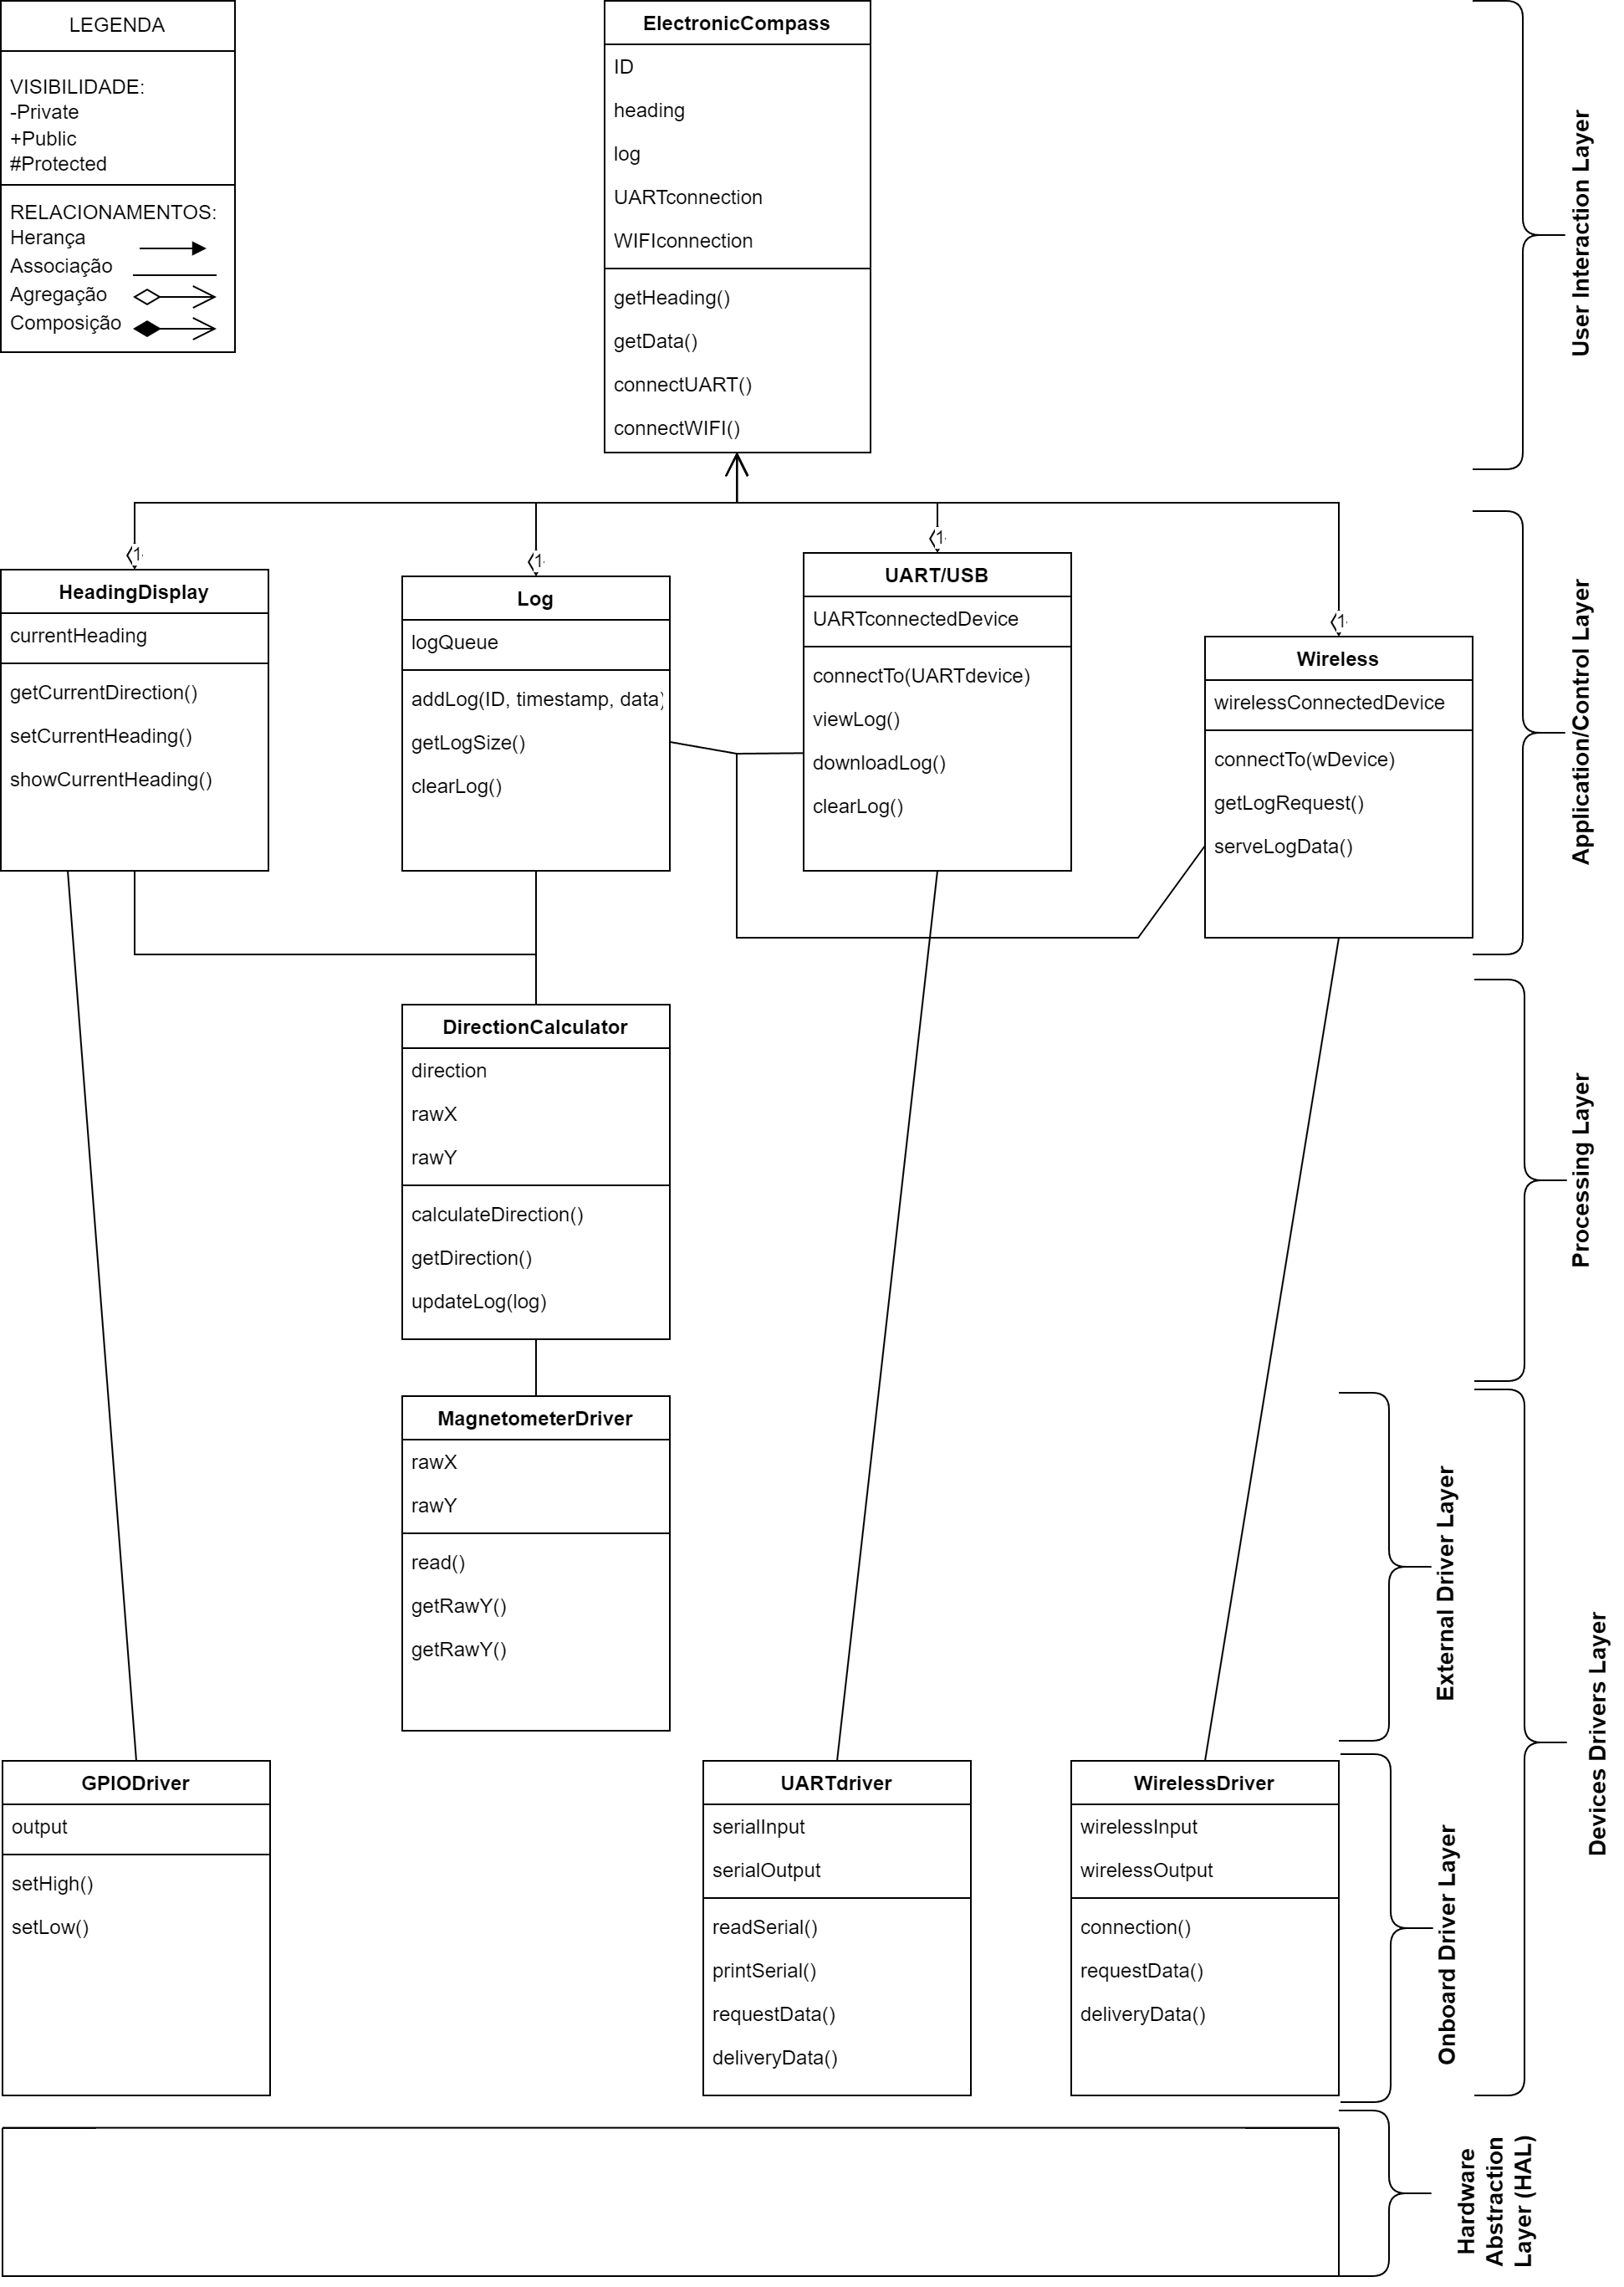
\includegraphics[keepaspectratio=true,scale=0.53]{figures/Diagrama_Classe_Projeto_Final_rev2.png}
  \caption{Diagrama de classes revisado do projeto organizado em camadas.}
  \label{fig:diagrama-classes}
\end{figure}

\onecolumn
\appendix{Apêndice B}
\label{apendice-b}

\subsection*{Diagrama de classes do projeto do \emph{Host}}
\begin{figure}[h]
  \centering
  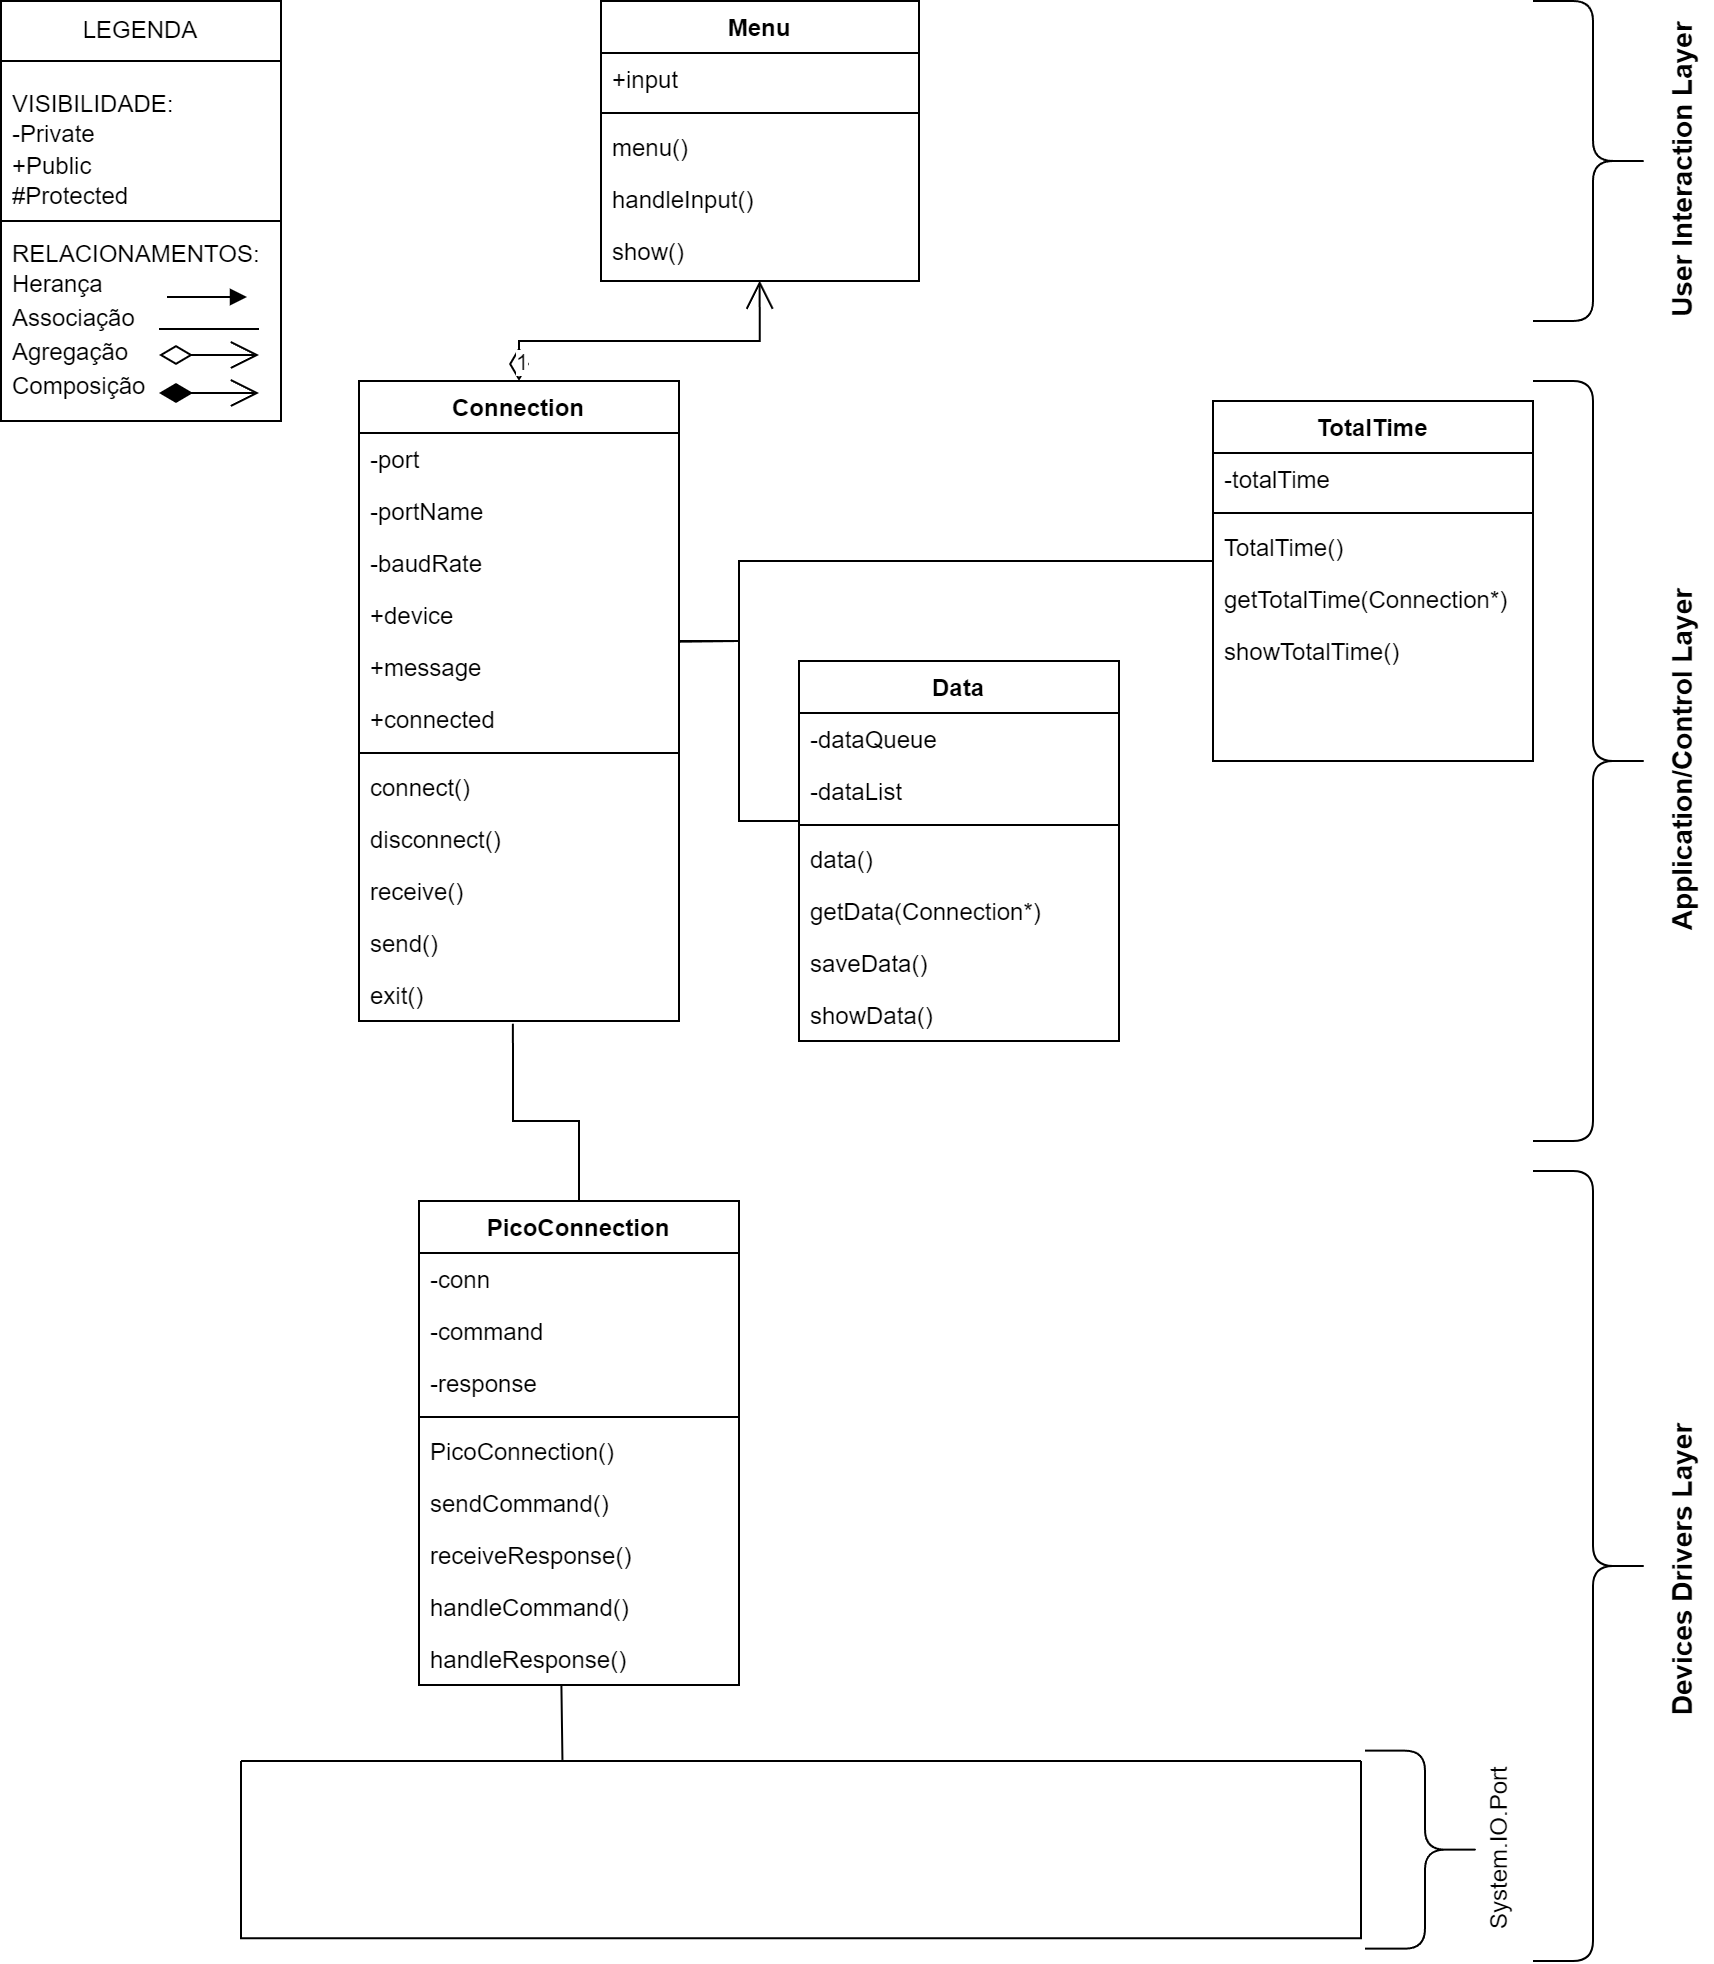
\includegraphics[keepaspectratio=true,scale=0.55]{figures/Diagrama_Classe_Host_PC.png}
  \caption{Diagrama de classes do projeto do \emph{Host}.}
  \label{fig:diagrama-host}
\end{figure}

\onecolumn
\appendix{Apêndice C}
\label{apendice-c}

\subsection*{Montagem dos módulos do Projeto}
\begin{figure}[h]
  \centering
  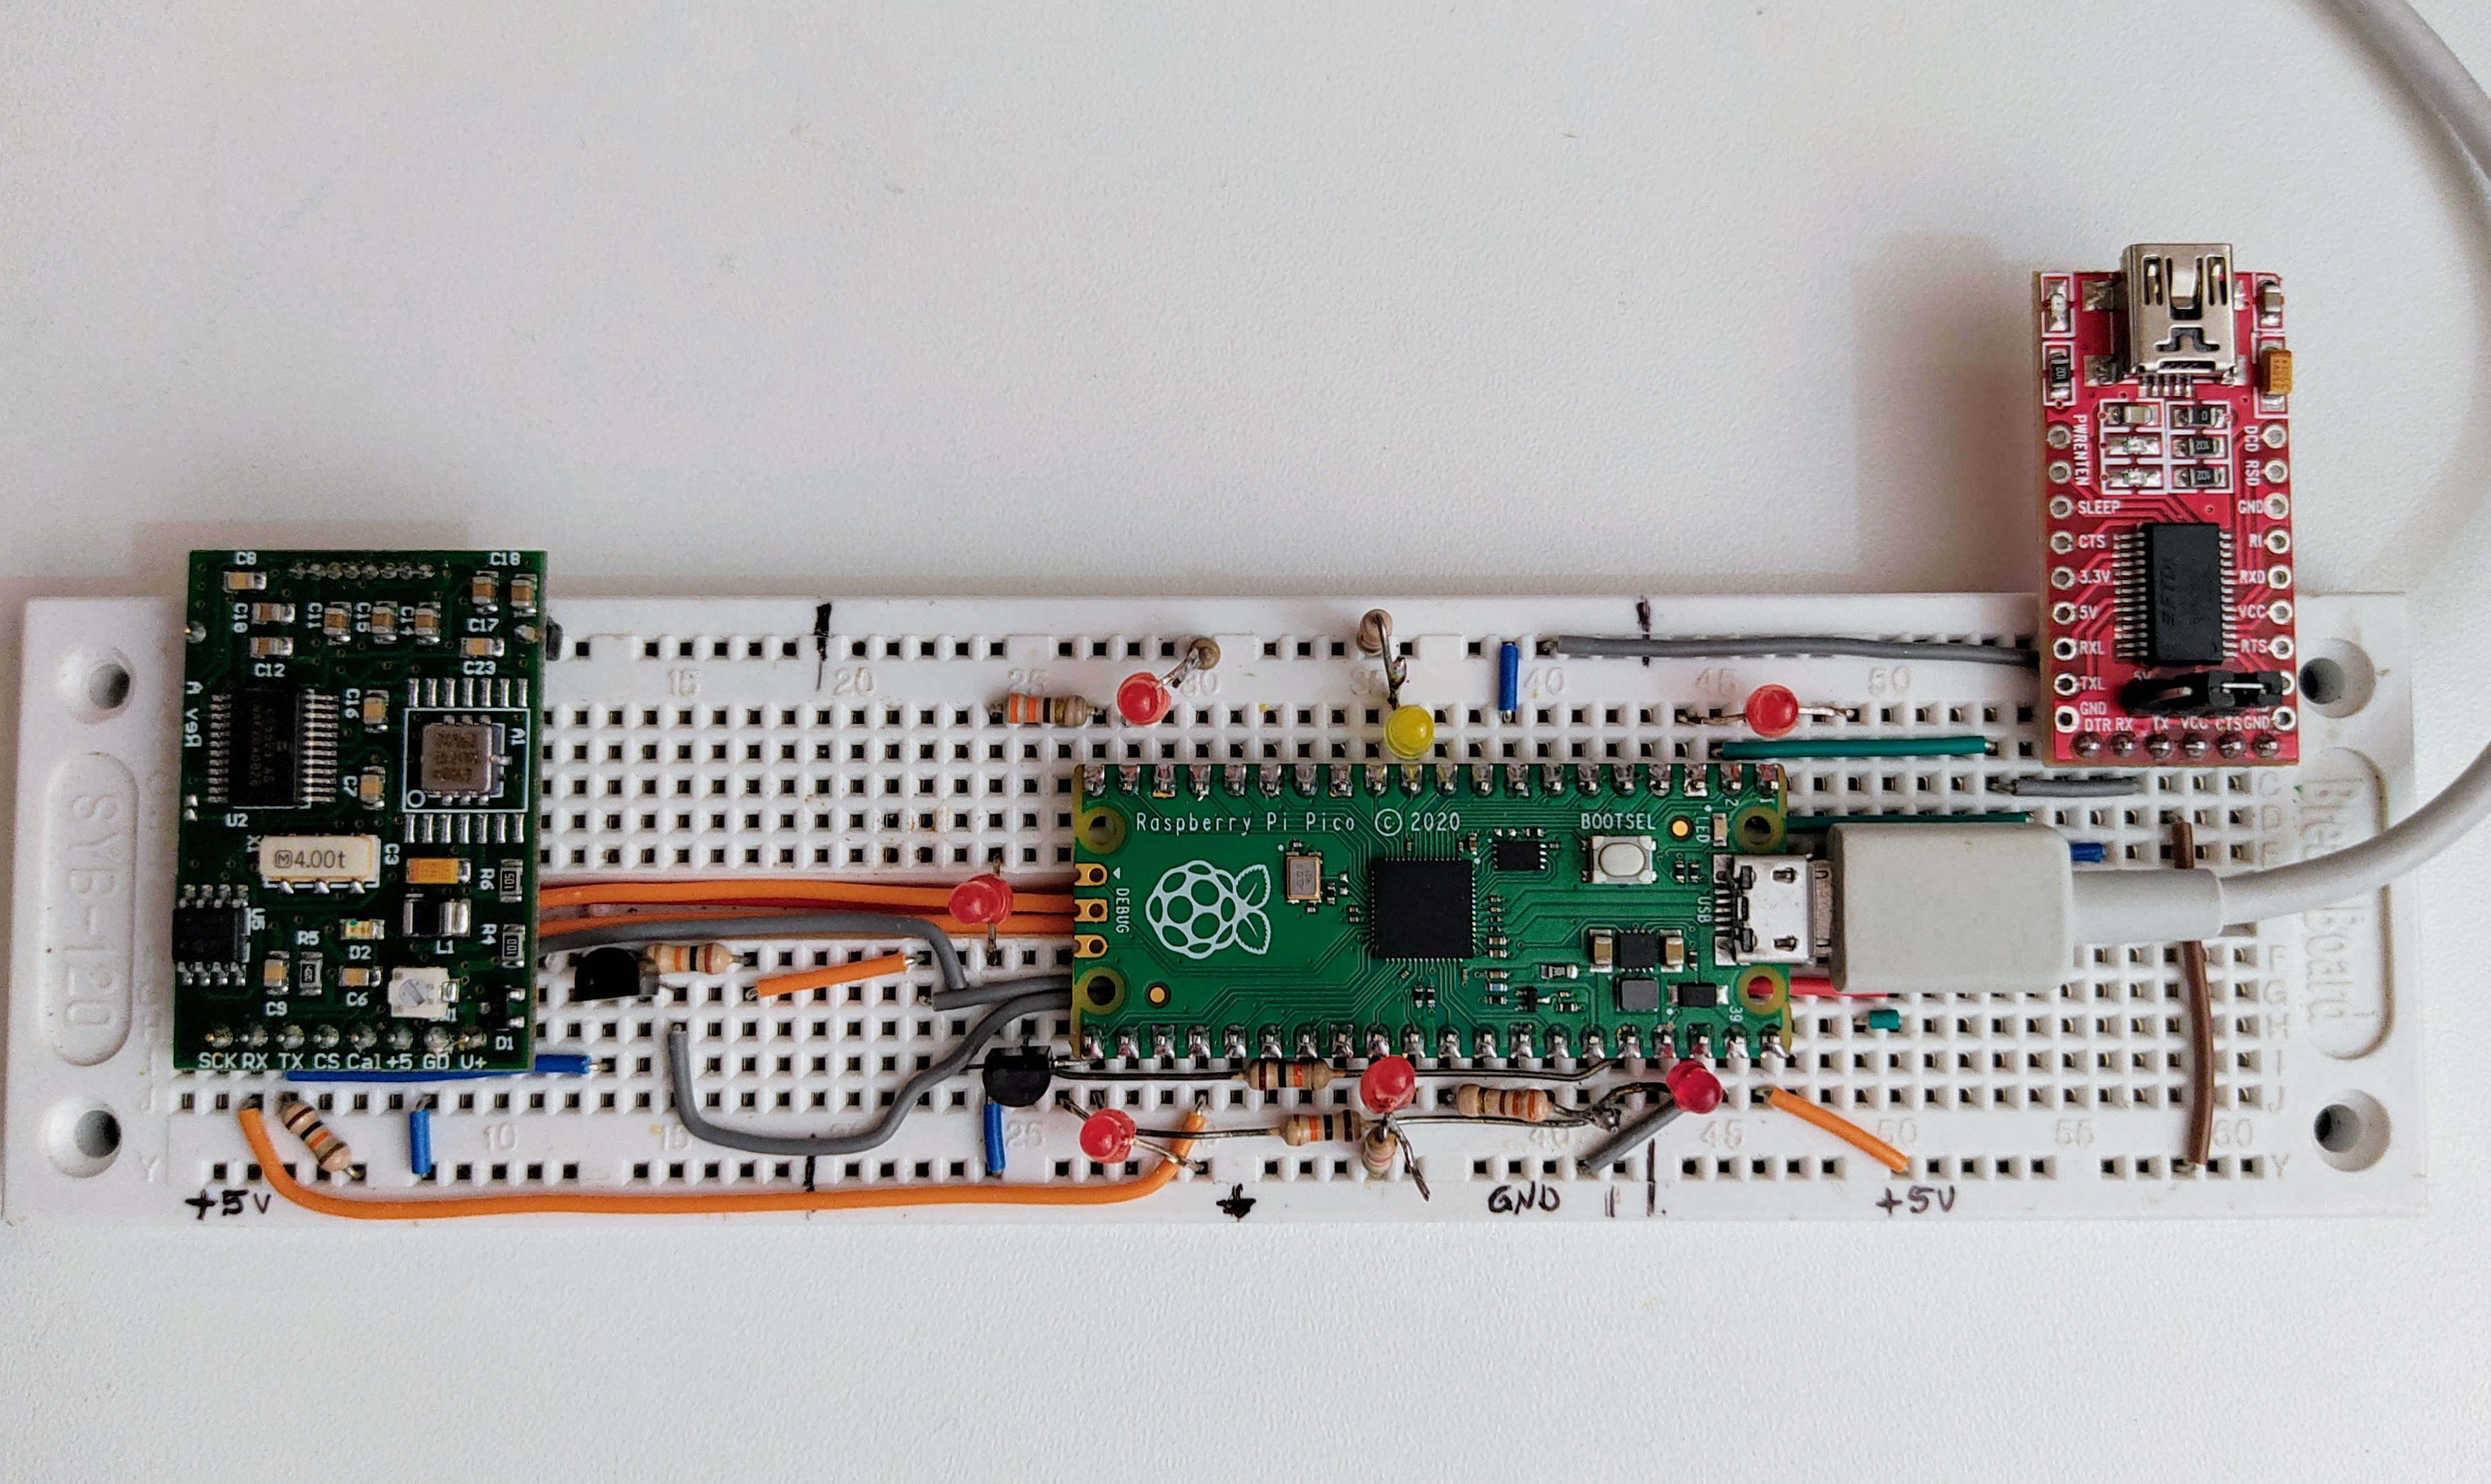
\includegraphics[keepaspectratio=true,scale=0.12]{figures/montagem.jpg}
  \caption{Montagem dos módulos do projeto.}
  \label{fig:montagem}
\end{figure}

\onecolumn
\appendix{Apêndice D}
\label{apendice-d}

\subsection*{Plano de testes da Bússola eletrônica de 2 Eixos}
\begin{figure}[h]
  \centering
  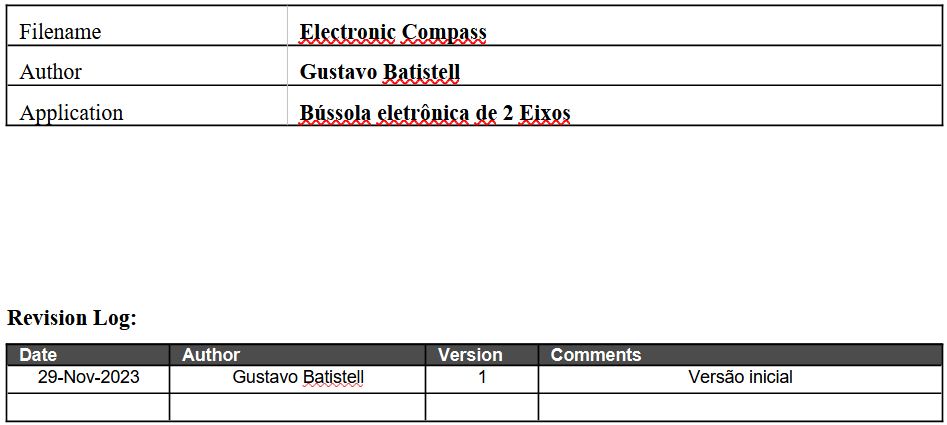
\includegraphics[keepaspectratio=true,scale=0.44]{figures/PlanoTestes.png}
 % \caption{Diagrama de classes do projeto organizado em camadas.}
  \label{fig:plano-testes}
\end{figure}

\subsection*{Introdução}
O objetivo desse plano de teste é orientar o teste de funcionamento do sistema Bússola Eletrônica	de 2 Eixos e suas partes.
\subsection*{Ambiente}
Uso de computador tipo PC rodando máquina virtual WSL Ubuntu no sistema operacional Windows 10 ou 11.
\subsection*{Processo}
\begin{itemize}
  \item Ligar o computador
  \item Rodar o WSL
  \item Clonar o repositório \cite{src-github} para a pasta local HOME.
  \item Entrar na pasta ~/ElectronicCompass\$ 
  \item Rodar a aplicação com o comando pcHost
\end{itemize}

\subsection*{Testes 1}
Resultados esperados:
\begin{itemize}
  \item Obter sucesso na conexão da comunicação
  \item Conseguir visualizar o tamanho do log de dados
  \item Visualizar os dados do período desejado
  \item Salvar os dados do período desejado
  \item Sair da aplicação com sucesso
\end{itemize}

\begin{itemize}
  \item Conferir exibição do menu de seleção na terminal
  \item Digitar a opção 1
  \item Verificar status da conexão
  \item Digitar a opção 2 para visualizar o tamanho do log de dados
  \item Digitar a opção 3 para visualizar os dados do log
  \item Digitar a opção 4 para salvar os dados do log
  \item Digitar a opção X para encerrar a aplicação
\end{itemize}

\end{document}
